\chapter{Telematik}

Zusammenfassung der Vorlesung "`Telematik"' aus dem Wintersemester 2016.\footnote{\url{https://telematics.tm.kit.edu/ws201617_telematik.php}}

\section{Transportprotokolle}

\subsection{Grundlegende Komponenten}

\subsubsection{TCP-Grundlagen}
\begin{itemize}
	\item \textbf{TCP-Verbindungsverwaltung}
	\begin{itemize}
		\item Identifikation einer TCP-Verbindung: Quell-/Zieladresse sowie Quell-/Zielport
		\item Verbindungsaufbau: Server wartet, Client initiiert Verbindung
		\item 3-Wege-Handshake
		\begin{enumerate}
			\item Client \(\rightarrow\) Server: \texttt{TConReq(SYN=1,seq=client\_isn)}
			\item Client \(\leftarrow\) Server: \texttt{TConCnf(SYN=1,ACK=1,seq=server\_isn,ack=client\_isn+1)}
			\item Client \(\rightarrow\) Server: \texttt{ACK(SYN=0,ACK=1,seq=client\_isn+1,ack=server\_isn+1)}
		\end{enumerate}
		\item Zusätzlich: Festlegen der initialen Sequenznummer (\texttt{isn}), Bekanntgabe der Größe des Flusskontrollfensters, Allokation der Puffer
		\item Format einer TCP-Dateneinheit\footnote{\url{https://upload.wikimedia.org/wikipedia/de/f/fd/TCP_Header.svg}}\\
			\begin{minipage}{\linewidth}
				\includegraphics[scale=0.38]{telematik/TCP_Header.pdf}
			\end{minipage}
	\end{itemize}
	\item \textbf{Flusskontrolle zur Schutz des Empfängers vor zu hoher Last}
	\begin{itemize}
		\item Dynamische Anpassung des Empfangsfenster auf Empfängerseite, um die aktuelle verfügbare Puffergröße mitzuteilen. \texttt{RcvWindow} bezeichnet den Anteil des \texttt{RecvBuffer}, das frei ist (jeweils absolute Werte)
		\item Problem: Empfänger meldet ein volles Empfangsfenster. Woher weiß der Sender, ab wann er wieder senden darf? \(\rightarrow\) Empfänger muss auch bei vollem Empfangsfenster Dateneinheiten mit einem Byte Länge quittieren (\textit{Zero Window Probing})
	\end{itemize}
	\item \textbf{Angriffe auf den Verbindungsaufbau: SYN-Flooding}
	\begin{itemize}
		\item Massenhaftes Senden von SYN-Dateneinheiten ohne Verbindungsaufbau. Problem: Zustandshaltung auf Empfängerseite für halboffene Verbindungen. Folge: Ressourcen erschöpft, Empfänger kann keine Dateneinheiten mehr annehmen
		\item Lösung: SYN-Cookies
		\begin{itemize}
			\item Verhinderung der Zustandshaltung bis zum letztmöglichen Zeitpunkt: Beginn der Zustandhaltung erst bei Empfang des \texttt{ACK}
			\item Realisierung: Ermittlung der Zustandsinformationen auf Empfängerseite anhand der Informationen aus \texttt{ACK(SYN=0,ACK=1,seq=client\_isn+1,ack=server\_isn+1)}
			\item Kodierungsbeispiel: Zeitstempel zur Verhinderung von Replay-Attacken (5 Bit); ausgewählte MSS aus acht vordefinierten Werten (3 Bit); Hash über Quelladresse und -port sowie Zieladresse und -port, verifiziert, dass der Client bereits \texttt{SYN} durchgeführt hat /24 Bit). Daraus entsteht die 32 Bit initiale Sequenznummer des Servers
			\item Nachteil: Vergleichsweise kurze Sequenznummer (32 Bit) reicht nicht für zusätzliche TCP-Optionen und limitiert MSS-Größen auf vordefinierte Werte
			\item Idee: Cookie erst einsetzen, wenn nötig (volle Warteschlange oder Ressourcenengpass)
		\end{itemize}
	\end{itemize}
\end{itemize}

\subsubsection{Staukontrolle}
\begin{itemize}
	\item Beobachtung: Unverhältnismäßiger Leistungseinbruch an Engstellen bei großem Datenaufkommen zwischen zwei schnelleren Netzen \(\rightarrow\) Warteschlangenmanagement notwendig
	\item \textbf{Einfaches Warteschlangenmanagement}
	\begin{itemize}
		\item Puffer im Router voll, nächste Dateneinheit muss verworfen werden ("`Tail Drop"')
		\item Retransmissiontimer im Client steuert Sendewiederholungen
		\item Problem: Synchronisation. Dateineinheiten von mehreren Verbindungen werden quasi gleichzeitig verworfen
	\end{itemize}
	\item \textbf{Aktives Warteschlangenmanagement}
	\begin{itemize}
		\item Das Netz gibt einen Hinweis auf eine entstehende Stausituation, bevor eine Überlast entsteht
		\item Router verwirft (randomisiert) Dateneinheiten, bevor die Warteschlange voll ist. Sorgt für Fairness und verhindert globale Synchronisation
		\item Verfahren
		\begin{itemize}
			\item Konkrete Implementierung: Random Early Detection (RED). Wahrscheinlichkeit, dass eine Dateneinheit verworfen wird, steigt linear mit der Warteschlangenlänge
		\end{itemize}
	\end{itemize}
	\item \textbf{Self-Clocking}: Verbindung zweier Netze über langsames Weitverkehrsnetz. Dateneinheiten benötigen bei der langsamen Übertragung mehr Zeit als in den lokalen Netzen. Dadurch kommen sie verzögert beim Empfänger an, welcher sie entsprechend "`langsam"' quittiert. Durch den entstehenden Takt weiß der Sender, wie schnell er senden kann. Aber: Wie soll die "`Uhr"' gestartet werden?
	\item Wieso wird trotzdem kein Gleichgewicht erreicht?
	\begin{itemize}
		\item Verbindung kommt nicht ins Gleichgewicht. Mögliche Auslöser: Neue Verbindung/Neustart, automatische Anpassung der Datenrate und Verzögerung \(\rightarrow\) Slow-Start
		\item Sender sendet neue Dateneinheiten zu früh \(\rightarrow\) Zeitgeber
		\item Ressourcenbeschränkungen verhindern Gleichgewicht \(\rightarrow\) Congestion-Avoidance
	\end{itemize}
	\item \textbf{Slow-Start (Einzelverbindung)}
	\begin{itemize}
		\item Erhöhung der Anzahl der gesendeten Dateneinheiten über die Zeit durch Einführung eines Staukontrollfensters (\texttt{Staukontrollfenster < Flusskontrollfenster}). Verhindert burstartiges Senden der Quelle, was zu vielen Sendewiederholungen führen würde
		\item Bei Verbindungsstart oder Verlust einer Dateneinheit wird das Staukontrollfenster zurückgesetzt
		\item Startverhalten ohne Slow-Start: Viele Sendewiederholungen durch Paketverluste. "`lineares Zickzackwachstum"', das weit hinter der verfügbaren Datenrate zurück bleibt (effektive Nutzung bei 35\%)
		\item Startverhalten mit 2s Slow-Start: Keine Sendewiederholungen, Datenrate nahezu am verfügbaren Maximum; Effizienz abhängig von Verbindungsdauer, da dann die langsame Slow-Start-Phase an Gewicht verliert
	\end{itemize}
	\item \textbf{Congestion Avoidence (Simultane, konkurrierende Verbindungen)}
	\begin{itemize}
		\item Ohne Congestion Avoidance: Sehr viele Sendewiederholungen (nahezu 50\% im Experiment), sehr unfaire Aufteilung
		\item Mit Congestion Avoidance: Sehr wenige Sendewiederholungen, verschiedene Quittungsstrategien möglich
		\item Zusammenfassung: Faire Aufteilung der verfügbaren Kapazität, langsames Herantasten durch lineares Erhöhen des Staukontrollfensters sowie kaum Sendewiederholungen
	\end{itemize}
	\item \textbf{Fast Retransmit}
	\begin{itemize}
		\item Beobachtung: Nicht jede nicht in Reihenfolge erhaltene Dateneinheit ist ein Indiz für eine Überlastung des Netzes
		\item Mechanismus zur Staukontrolle: Sendewiederholung beim Empfang einer definierten Anzahl duplizierter Quittungen (letztere entstehen dadurch, das der Empfänger immer das neuste, lückenlos übertragene Paket quittiert)
		\item Vorgehen: Warten auf Timerablauf, dann Sendewiederholung (Wartezeit \(>\) \texttt{RTT})
	\end{itemize}
	\item \textbf{Staukontrolle}
	\begin{itemize}
		\item Implizite Staukontrolle: "`Anzeigen"' einer Stausituation ohne explizite Unterstützung des Netzes
		\begin{enumerate}
			\item TCP-Tahoe
			\begin{itemize}
				\item Mechanismen: Slow Start, Timeout, Congestion Avoidance, Fast Retransmit
				\item Nach Timeout oder Empfang duplizierter Quittungen: Beginn von Slow Start
				\item Grundlegende Vorgehensweise: Additives Erhöhen des Congestion Window \texttt{CWnd}, multiplikatives Verringern (\texttt{AIMD})
			\end{itemize}
			\item TCP-Reno
			\begin{itemize}
				\item Zusätzlich zu TCP-Tahoe: Fast Recovery (siehe unten)
				\item Unterscheidet zwischen \textit{schweren Stausituationen} (Timeout bei ausstehenden Quittungen) und \textit{leichten Stausituationen} (Empfang von duplizierten Quittungen)
				\item Leichte Stausituationen: Kein Rücksetzen auf Slow Start, da Quittungsempfang impliziert, dass weiter neue Daten empfangen worden sind \(\rightarrow\) Fast Recovery
				\item Schwere Stausituationen: Rücksetzen auf Slow Start wie bei TCP-Tahoe
				\item Fast Recovery
				\begin{itemize}
					\item Szenario: Empfang einer festgelegten Anzahl Quittungen (beispielsweise drei)
					\item Idee: Senden neuer Dateneinheiten, auch wenn der Fehler noch nicht behoben ist (Self-Clocking geht weiter)
					\item Vorgehen: Reduzierung der Belastung (halbieren des Staukontrollfensters) sowie Fast Retransmit
				\end{itemize}
			\end{itemize}
		\end{enumerate}
		\item Explizit Congestion Notification (ECN): Explizite Staukontrolle mit Netzunterstützung
		\begin{itemize}
			\item Idee: Erkennen von Stausituationen im Netz über den Füllstand der Warteschlange (setzt aktives Warteschlangenmanagement voraus) sowie Markieren der IP-Einheiten vor Weiterleitung zum Empfänger. Dieser informiert den Sender, um das Staukontrollfenster zu regeln
			\item Signalisierung in Schicht 3 (IP): Nutzung zweier ehemaliger Bits im \texttt{ToS}-Feld der Dateneinheit
			\begin{description}
				\item{\texttt{ECT}-Bit}: Aktiviert ECN
				\item{\texttt{CE}-Bit}: Zeigt an, ob gerade Stau ist
			\end{description}
			\item Signalisierung in Schicht 4 (TCP): Einführung zusätzlicher Flags im TCP-Kopf
			\begin{description}
				\item{\texttt{ECE}-Bit}: Signalisiert dem Sender die Stausituation (Sender \(\leftarrow\) Empfänger)
				\item{\texttt{CWR}-Bit}: Bestätigt dem Empfänger den Erhalt einer Staumeldung (Sender \(\rightarrow\) Empfänger)
			\end{description}
			\item Vorgehen: Infrasturktur signalisiert in Schicht 3 auf dem Weg zum Empfänger, dass eine Stausituation besteht; Empfänger signalisiert darauf hin dem Sender die Stausituation in Schicht 4, dieser handelt entsprechend (halbiert \texttt{CWnd}, reduziert \texttt{SSTresh}) und bestätigt die Staumeldung explizit
		\end{itemize}
	\end{itemize}
\end{itemize}

\subsubsection{Fairness}
\begin{itemize}
	\item TCP-Verbindungen konkurrieren um Ressourcen des Netzes \(\rightarrow\) faire Aufteilung angestrebt
	\item \textbf{Probleme}
	\begin{itemize}
		\item "`Gierige Nutzer"': Faire Verteilung bezieht sich auf TCP-Verbindungen. Kann daher mehrere Verbindungen gleichzeitig öffnen. Gegenmaßnahme: Verteilung der Kapazität pro Benutzer
		\item "`Gieriger Empfänger"': Da das Quittungsverhalten der Empfängerinstanz die Ressourcenzuteilung beeinflusst, kann dieser mehr oder weniger schell Quittungen senden. Das Staukontrollfenster öffnet sich schneller, damit erhält die Verbindung mehr Ressourcen
		\begin{enumerate}
			\item Mehrere Quittungen pro empfangener Dateneinheit: Sequenznummern zählen Bytes, Staukontrollfenster zählen Dateneinheiten. Bestätigt der Empfänger jede Dateneinheit in mehreren "`Häppchen"', so öffnet sich das Staukontrollfenster schneller
			\item Quittungen schneller senden als Daten empfangen werden. Protokolländerung notwendig
			\item Identische Quittungen mehrfach senden: Fehlende Dateneinheit wird erneut gesendet. Bei TCP-Reno läuft Self-Clocking weiter \(\rightarrow\) Staukontrollfenster wird weiter geöffnet
		\end{enumerate}
	\end{itemize}
\end{itemize}

\subsection{Analyse und Randbedingungen}

\subsubsection{Analyse von TCP: Modelle}
\begin{itemize}
	\item Analytische Beurteilung hinsichtlich Durchsatz und Latenz
	\item Zentrale Fragen: Ist \texttt{TCP} für meine Zwecke geeignet "`Welche Leistung kann ich erwarten?"'
	\item \texttt{Periodisches Modell}
	\begin{itemize}
		\item Vereinfachte Betrachtung des langfristigen Verhaltens ohne Slow-Start und Sendewiederholungen \(\rightarrow\) Staukontrollfenster bildet "`perfekte"' Sägezahnkurve mit periodischen Paketverlusten
		\item Vorgehen: Berechne die Anzahl übertragender Dateneinheiten \(Y_i\) zwischen zwei aufeinenader folgenden Verlusten von Dateneinheiten (also in einem Durchlauf)
		\item Durchschnittliche Übertragungsrate: \(X=\frac{1}{RTT}\cdot\sqrt{\frac{3}{2p}} = 1,22 \cdot \frac{1}{RTT\cdot\sqrt{p}}\)
		% TODO: Relevanz?
	\end{itemize}
	\item \texttt{Detailliertes Verlust-Modell}
	\begin{itemize}
		\item Unterschied zum periodischen Modell: Verluste nicht mehr periodisch \(\rightarrow\) Dauer der Durchläufe nicht mehr gleich lang
		% TODO: Relevanz?
	\end{itemize}
\end{itemize}

%\subsubsection{Hohe Datenraten}
% TODO: Relevanz?

\subsubsection{Kurze Latenzen: TCP und Web}
\begin{itemize}
	\item Interaktiver Dienst, Besucher äußerst ungeduldig \(\rightarrow\) Antwortzeit entscheident
	\item Verwendung von \texttt{HTTP} in \texttt{TCP} \(\rightarrow\) bei jedem Klick/pro Objekt wird mindestens eine \texttt{TCP}-Verbindung aufgebaut \(\rightarrow\) sehr viele Verbindungsaufbauten für wenig Übertragung
	\item Bei kleinen Objekten dominieren RTTs die Antwortzeit; Slow-Start hat entscheidenden Einfluss auf die Verzögerung
	\item \textbf{Möglichkeiten zur Verbesserung}
	\begin{itemize}
		\item Größeres initiales Staukontrollfenster: Mindestens 10 \texttt{TCP}-Segmente mit \(\sim 15\) KByte, da 90\% aller Web-Objekte \(\le 16\) KByte sind. Google-Messungen (in kleiner Umgebung) bestätigen die Vermutung, wobei das initiale Staukontrollfenster auch nicht zu groß werden darf
		\item TCP-Fast-Open (TFO): Verzögerungsreduzierung beim Verbindungsaufbau, da bereits im \texttt{SYN}-Paket Daten ausgeliefert werden, die allerdings erst nach dem kompletten Handshake an die Anwendung ausgeliefert werden \(\rightarrow\) verkürzt die Latenz um eine \texttt{RTT}, eröffnet aber auch die Möglichkeit für DoS-Attacken mittels \texttt{SYN}-Flooding \(\rightarrow\) TFO-Cookie als mögliche Lösung
	\end{itemize}
\end{itemize}


\subsection{Aktuelle Entwicklungen}

\subsubsection{Realität im Internet}
\begin{itemize}
	\item Datentransport nicht mehr nur klassischerweise zwischen Endgeräten, die über Routern kommunizieren. Paradigma: \texttt{IP}-Dateneinheiten werden nicht modifiziert \(\rightarrow\) beliebige Transportprotokolle nutzbar
	\item Praktisch greifen jede Menge Middleboxes in den E2E-Datenstrom ein und können fast alle Felder einer \texttt{TCP}-Dateneinheit verändern \(\rightarrow\) keine E2E-Transparenz mehr. Beispiele: Physikalische (Hardware-Firewall) oder virtuelle (NAT in Heimroutern, Software-Firewall) Firewalls modifizieren Einheiten. Datenpfade ohne Middleboxes eher die Ausnahme
	\item Network Address Translation (NAT) für maskierte Netze. NAT-Router ersetzt ausgehende Pakete durch seine Adresse und speichert das Mapping zum Zuordnen von Antworten. NAT-Router muss hierfür das Transportprotokoll kennen
	\item \textbf{Firewall}
	\begin{itemize}
		\item Untersuchen Dateneinheiten nach konfigurierten Regeln und verwerfen diese ggf.
		\item \textit{Shallow Packet Inspection}: Bewertung anhand des \texttt{IP}-Kopfs und den Köpfen der Transportprotokolle
		\item \textit{Deep Packet Inspection}: Anwendungsorientierte Bewertung, beispielsweise das Erkennen und Blockieren von Malware
	\end{itemize}
	\item \textbf{Proxy}
	\begin{itemize}
		\item Führen Kommunikation anstatt des Clients durch
		\item Können Ressourcen zwischenspeichern; Anfragen ablehnen/verändern; Logs anlegen
		\item Häufig: Sperren mittels Firewalls, Erlauben mittels Proxys
		\item Nicht-transparent (kann sich Servern gegenüber zu erkennen geben) oder transparent (benötigt Unterstützung der Netzwerkinfrastruktur, häufig zur Überwachung eingesetzt)
	\end{itemize}
	\item \textbf{Load-Balancer}
	\begin{itemize}
		\item Verteilt Anfragen/Berechnungen auf verschiedene, nachgelagerte Server, oft kombiniert mit vorgelagerten Caches
		\item Erscheint als Ziel-Adresse eines Services ("`umgedrehtes"' NAT)
	\end{itemize}
	\item Cache: Schnelle Auslieferung häufig angefragter Daten, oft in Kombination mit einem Proxy
	\item \textit{Head-of-Line Blocking}: Zuverlässiger Transportdienst blockiert auf Grund von fehlenden Dateneinheiten (Reihenfolgetreue) \(\rightarrow\) Daten werden nicht an Anwendung ausgeliefert. Bei Multimediakommunikation und im Web nicht erwünscht (interaktiver Dienst, Antwortzeit entscheident)
	\item \textbf{SPDY und HTTP/2}
	\begin{itemize}
		\item \texttt{SPDY} zunächst von Google zum teilweise Ersetzen von \texttt{HTTP} (Weiterentwicklung durch \texttt{IETF} zu \texttt{HTTP/2})
		\item Ziele
		\begin{itemize}
			\item Kurze Antwortzeiten: Eine dauerhafte \texttt{TCP}-Verbindung pro Server; Priorisierung von Anfragen; Server-Push; effizientere Header-Kodierung (vereinfacht, binär und komprimiert)
			\item Verbesserte Sicherheit: \texttt{TLS} verpflichtend 
			\item Rückwärtskompatibilität
		\end{itemize}
		\item Probleme: Kleine initiale Staukontrollfenster behindern \texttt{SPDY}; Slow-Start-After-Idle ruiniert Langzeitverbindungen; Head-of-Line Blocking durch verlorene Dateneinheiten
	\end{itemize}
	\item \textbf{Quick UDP Internet Connections (QUIC)}
	\begin{itemize}
		\item Ziele: Vermeidung von Head-of-Line Blocking; Reduzierung der \texttt{RTT}
		\item Einbettung zwischen \texttt{UDP} und \texttt{SPDY} bzw. \texttt{HTTP/2}
		\item Wichtige Eigenschaften: Schneller (\texttt{0-RTT}) Verbindungsaufbau; Vorwärtsfehlerkorrektur auf Ebene der Dateneinheiten; eigene Staukontrolle
	\end{itemize}
\end{itemize}

\subsubsection{TCP in Datenzentren}
\begin{itemize}
	\item Extrem hohe Anforderungen an Leistungsfähigkeit der Kommunikationssysteme; häufig Nutzung von Commodity-Netzen; Fat-Tree-Topologie (siehe Datacenter-Ethernet)
	\item \textbf{Typische Eigenschaften}
	\begin{itemize}
		\item Geringe Umlaufzeit durch geografische Nähe
		\item Incast-Kommunikation (Many-To-One): Mehrere Quellen senden zu einer Senke. Beim parallelen Laden zusammenhängender Daten bestimmt die langsamste Verbindung die Geschwindigkeit (Barrier Synchronization) \(\rightarrow\) Staugefahr am Switch
		\item Multiple Paths zwischen Servern
		\item Mischung von langen und kurzen Flows
		\item Virtualisierung
	\end{itemize}
	\item Data-Center-TCP: Konstant kurze Warteschlangen bei Switches durch \texttt{ECN} und reduzierte Staukontrollfenster beim Sender
\end{itemize}

\subsubsection{Multipath-TCP (MPTCP)}
\begin{itemize}
	\item \textbf{Motivation}
	\begin{itemize}
		\item Mobile Geräte haben typischerweise mehrere Netzwerkgeräte (WLAN, Ethernet, 3G, etc.); redundante Pfade in Datenzentren; Multi-Homing für Serverfarmen \(\rightarrow\) \texttt{TCP}-Verbindungen sollten zwischen Netzwerkgeräten migriert werden können
		\item \texttt{TCP} ist durch statische Identifikation (Adressen, Ports) ein \textit{Single-Path Protokoll}
	\end{itemize}
	\item Ziel: \texttt{TCP} zur Nutzung mehrerer Pfade erweitern; Anwendungskompatibilität und Netzwerkompatibilität sollen erhalten bleiben
	\item Herausforderung: Middleboxen, die Zustände halten
	\item \textbf{Architektur}
	\begin{description}
		\item{\texttt{MPTCP}-Verbindung}: E2E-Kommunikationsbeziehung; besitzt ein oder mehrere \texttt{MPTCP}-Subflows
		\item{\texttt{MPTCP}-Subflow}: Ein konkreter Pfad; entspricht einer "`regulären"' \texttt{TCP}-Verbindung; können dynamisch zu einer \texttt{MPTCP}-Verbindung hinzugefügt/gelöscht werden
		\item{OSI-Schicht}: Neue Subschicht oberhalb von \texttt{TCP} ("`Management der Multipath-Verbindung"')
	\end{description}
	\item Weitere Details: Ein Gesamt-Eingangspuffer für alle Subflows; Subflow-Scheduling; Subflow-Staukontrolle
\end{itemize}



\section{Routing im Internet}

\subsection{Grundlagen}
\begin{itemize}
	\item Aufgaben: Weiterleitung sowie Kopplung von Netzen \(\rightarrow\) Verknüpfung einzelner Übertragungsabschnitte zu einer E2E-Übertragung
	\item Wegfindung im Kommunikationssystem: Weiterleitung im Router anhand Weiterleitungstabelle. Schnelle Weiterleitung mittels kurzer Warteschlangen und kleinen Tabellen
	\begin{itemize}
		\item Pro Dateneinheit ein Lookup in Weiterleitungstabelle
		\item \textit{Metriken} (üblicherweise Ganzzahl) zur Bewertung von Übertragungsabschnitten
		\item \textit{Policies} als Betreibervorgabe zur Routingstrategie. Bsp.: "`Bevorzugt bestimmten Nachbarn wählen"'
	\end{itemize}
	\item Herausforderung: Weiterleitung in Line-Speed. Dazu extrem teure, spezielle Cisco Hardware mit bis zu \texttt{1,2 Tbit/s} pro Chassi \(\rightarrow\) nur wenige dutzend Nanosekunden Bearbeitungszeit pro Dateneinheit
	\item Das Internet Protokoll (IP): Unzuverlässiger Dienst; keine Kontexthaltung in Zwischensystemen; keine Verbindungen
\end{itemize}

\subsubsection{Router}
\begin{itemize}
	\item \textbf{Weiterleitung}
	\begin{itemize}
		\item Aufbau Weiterleitungstabelle: \(Prefix \rightarrow Port\) mit Default-Regel am Ende (falls keine der oberen Regeln zutrifft)
		\item Falls mehrere Einträge passen: \textit{Longest Prefix Matching}
		\item Suche in Line-Speed: Verfahren
		\begin{itemize}
			\item Binärer Trie: Pfadabstieg entsprechend den Adressbits
			\item Patricia Trie zur komprimierten Speicherung von Binärbäumen: Knoten ohne Verzweigung überspringen und dabei Index vom nächsten relevanten Bit merken
			\item Problem bei Bäumen: Eintrag im Worst-Case in \(\mathcal{O}(n)\)
			\item Hash-Tabelle zur Beschleunigung des Lookups
			\begin{itemize}
				\item Longest-Prefix nicht praktikabel \(\rightarrow\) Suche nach der kompletten Adresse
				\item Trie-Lookups lediglich, wenn kein Eintrag in der Hashtabelle vorhanden ist
			\end{itemize}
			\item Hardwarerealisierung \textit{Content-Addressable Memory} (CAM)
			\begin{itemize}
				\item Speicherzugriff über einen Teil des gespeicherten Inhalts
				\item Sehr schnell, da in Hardware realisiert; paralleler Zugriff möglich
				\item Anwendung hier: Abbildung \(\big\lbrack IPAdresse \rightarrow Ausgangsport\big\rbrack\)
				\item Problem: Zuordnung einzelner Adressen wenig hilfreich. Daher \textit{Ternary Content-Addressable Memory} mit don't-care Bits \(\rightarrow\) Suche nach Präfixen möglich
			\end{itemize}
		\end{itemize}
		\item Aufgaben bei Weiterleitung: Header überprüfen; TTL aktualisieren; Prüfsumme neu berechnen; Lookup; Fragmentierung; Behandlung von IP-Optionen; ggf. Klassifizierung und Priorisierung
		\item Generische Router-Architektur: Der Routingprozessor behandelt lediglich die Kontrolldateneinheiten. Alle Komponenten außer der Routingprozessor puffern. Zielkonflikt Leistungsfähigkeit vs. Kosten\\\\
		\begin{figure}[!h]
		\centering
		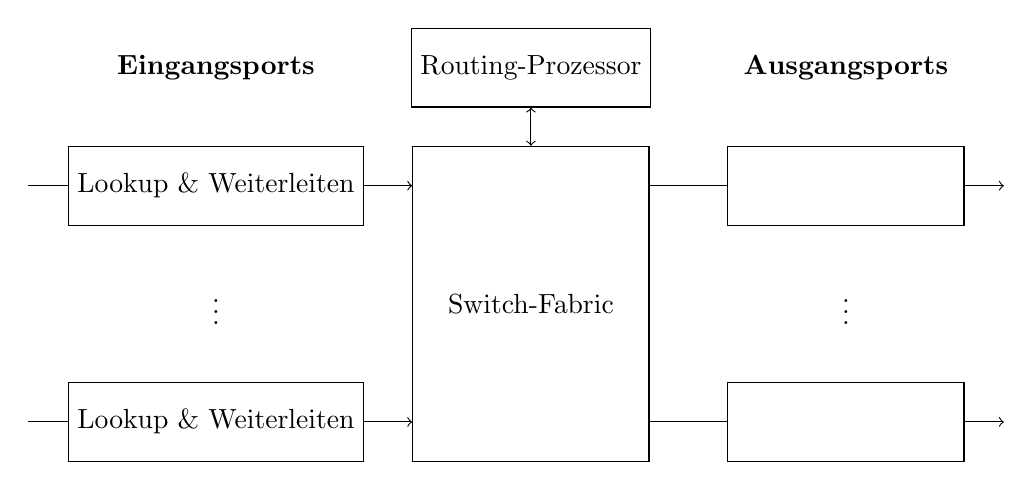
\begin{tikzpicture}
			\node at (4, -3)    [rectangle,draw,minimum height=4cm,minimum width=3cm] (sf)  {Switch-Fabric};
			\node at (4,  0)    [rectangle,draw,minimum height=1cm,minimum width=3cm] (rp)  {Routing-Prozessor};
			\node at (0, -1.5)  [rectangle,draw,minimum height=1cm,minimum width=3cm] (e1)  {Lookup \& Weiterleiten};
			\node at (0, -4.5)  [rectangle,draw,minimum height=1cm,minimum width=3cm] (en)  {Lookup \& Weiterleiten};
			\node at (8, -1.5)  [rectangle,draw,minimum height=1cm,minimum width=3cm] (a1)  {};
			\node at (8, -4.5)  [rectangle,draw,minimum height=1cm,minimum width=3cm] (an)  {};

			\node at (0, 0) {\textbf{Eingangsports}}; \node at (8, 0) {\textbf{Ausgangsports}};
			\node at (0, -3) {\(\vdots\)}; \node at (8, -3) {\(\vdots\)};

			\draw[<->] (sf) edge node {} (rp);
			\draw[-] (e1.west) -- ++(-0.5cm,0) |- (e1); \draw[->] (e1) edge node {} (e1-|sf.west);
			\draw[-] (en.west) -- ++(-0.5cm,0) |- (en); \draw[->] (en) edge node {} (en-|sf.west);
			\draw[-] (sf.east|-a1) edge node {} (a1);   \draw[->] (a1) -| (a1.east) -- ++(0.5cm,0);
			\draw[-] (sf.east|-an) edge node {} (an);   \draw[->] (an) -| (an.east) -- ++(0.5cm,0);
		\end{tikzpicture}
		\end{figure}
	\end{itemize}
	\item \textbf{Switch-Fabric}
	\begin{itemize}
		\item Blockierungen: Gegenmaßnahmen
		\begin{itemize}
			\item \textit{Overprovisioning}: Interne Verbindungen schneller als Eingangsports
			\item Pufferung an den Netzwerkschnittstellen und in Switch-Fabric. Annahmen zur Vereinfachung: Gleiche Datenrate an allen Ports; alle Pakete gleich groß
			\begin{itemize}
				\item Eingangspuffer: Konfliktauflösung am Eingang; geeignete Scheduling-Strategie
				\item Ausgangspuffer: Konfliktauflösung am Ausgang, allerdings \(N\)-fache Vermittlungsgeschwindigkeit der Eingangsports notwendig. Kurze Eingangspuffer zur Aufnahme von jeweils einer Dateneinheit trotzdem notwendig
				\item Verteilter Puffer pro Knotenpunkt in Switch-Fabric: Höherer Speicherbedarf
				\item Zentraler Puffer zur Konflikauflösung: Geringerer Speicher als bei den anderen Puffern nötig, allerfings höhere Anforderungen an die Speicherzugriffszeit 
			\end{itemize}
			\item Backpressur: Überlastsignalisierung an die Eingangsports \(\rightarrow\) Eingangsports reduzieren Last
			\item Parallele Switch-Fabrics
		\end{itemize}
		\item Struktur der Switch-Fabric
		\begin{itemize}
			\item Gemeinsamer Speicher
			\item Bus-/Ringstruktur: Konfliktfreier Zugriff durch Zeitmultiplex; \(\big\lbrack Uebertragungskapazitaet \ge \sum Kapazitaet-Eingangsport_i\big\rbrack \); Multicast und Broadcast trivial; Anzahl der Anschlüsse sehr begrenzt (\(\le 16\)); Bsp.: \texttt{CISCO 7500}
			\item Koppelmatrix: Alle Eingänge mit allen Ausgängen verbunden; teilweise parallel nutzbar; hoher Verdrahtungsaufwand; unflexibel; besonders effizient bei gleichgroßen Dateneinheiten
			\item Mehrstufige Verbindungsnetzwerke: Ebenfalls alle Eingänge mit allen Ausgängen durch hierarchische Schaltelemente verbunden; geringerer Verdrahtungsaufwand als Koppelmatrix; nicht alle Verbindungen gleichzeitig möglich
		\end{itemize}
	\end{itemize}
\end{itemize}

\subsubsection{Routing-Algorithmen}
\begin{itemize}
	\item Kontrollpfad: Austausch von Routingnachrichten zur Berechnung von Wegen; Routingprotokolle
	\item Datenpfad: Weiterleitung von IP-Paketen
	\item Routingtabelle: \(\big\lbrack Prefix \rightarrow Next~Hop\big\rbrack \); wird von den Routingalgorithmen erstellt; auf die Anforderungen von Routingalgorithmen optimiert
	\item Weiterleitungstabelle: \(\big\lbrack Prefix \rightarrow Ausgangsport\big\rbrack\); auf effizienten Lookup optimiert
	\item \textbf{Verteiltes Adaptives Routing}
	\begin{itemize}
		\item Router reagieren dezentral auf sich ändernde Netzsituation (Laständerungen, Linkfehler, etc.)
		\item Adaptiv: Verteiltes Routing mit Informationsaustausch zwischen den Routern
		\item Benötigte Komponenten: Monitoring, Informationsaustausch, Berechnung aktueller/alternativer Routen
	\end{itemize}
	\item \textbf{Distanzvektor vs. Link-State}
	\begin{itemize}
		\item Distanzvektor-Algorithmus: Iterative Berechnung der kürzesten Pfade (beispielsweise via Bellman-Ford-Algorithmus). Umsetzung als \textit{Router Information Protocol} (RIP) im Internet. Routinginformationen werden auf Basis der Informationen von den Nachbarn berechnet und ausgetauscht
		\item Link-State-Algorithmus: Globale Sicht zur Berechnung der kürzesten Pfade (Dijkstra-Algorithmus) \(\rightarrow\) jeder Router muss alle Links im Netz kennen \(\rightarrow\) Informationen über lokale Links eines Routers breiten sich im gesamten Netz aus; jeder Router berechnet kürzeste Wege selbstständig (replizierte Berechnung); im Internet als \textit{Open Shortest Path First} (OSPF) umgesetzt
	\end{itemize}
	\item \textbf{Historisches}
	\begin{description}
		\item{1. Generation}
		\begin{itemize}
			\item Dateneinheiten werden in Richtung mit geringster Verzögerung weitergeleitet (instantene Messung); basiert auf Bellman-Ford-Algorithmus
			\item Probleme: Langsame Anpassung bei geänderter Lastsituation; Schleifen und Oszillationen möglich; Skaliert nicht durch Versenden großer Routingtabellen; gemessene Verzögerungswerte schlecht zu bewerten
		\end{itemize}
		\item{2. Generation}
		\begin{itemize}
			\item Dateneinheiten entlang der geringsten, über 10s gemittelten Verzögerung; Dijkstra-Algorithmus
			\item Bessere Verzögerungswerte bei leichter Lastsituation
			\item Probleme: Routing-Oszillation; schlecht ausgelastete Routen
		\end{itemize}
		\item{3. Generation}
		\begin{itemize}
			\item Angepasste Metrik: "`Gute"' Pfade betrachten, statt "`den"' besten Pfad \(\rightarrow\) bessere Netzauslastung bei hoher Last
		\end{itemize}
	\end{description}
\end{itemize}

\subsubsection{Routing-Architektur}
\begin{itemize}
	\item Strukturierung in \textit{Autonome Systeme} mit externem (\texttt{Exterior Gateway Protocol}) und internem (\texttt{Interior Gateway Protocol}) Routing \(\rightarrow\) Skalierbarkeit durch zwei logische Ebenen
	\item Autonome Systeme: Erscheinen nach außen als Einheit mit einheitlichem internen Routingprotokoll und gleicherer internen Routingpolicy. IANA delegiert die Zuteilung
	\begin{itemize}
		\item Aufteilung nach Funktion: Stub-AS (kleines Unternehmen mit einem Provider); Multihomed AS (große Unternehmen mit mehreren Providern); Transit AS (Provider, oft global)
		\item Aufteilung nach Bedeutung: Transit AS/Tier-1 mit angeschlossenen Tier-2-Ebenen, etc.
	\end{itemize}
	\item Transit: Ziel ist Übertragungspfade zu allen am Internet teilnehmenden ASen herstellen. AS-Betreiber kauft hierzu die Konnektivität zu einem/mehrerer ASen ("`Durchgangsverkehr"') zu ASen, die nicht direkt angeschlossen werden können)
	\item \textbf{Peering}
	\begin{itemize}
		\item Private Peering: Direktverbindung zweier ASe, i.d.R. auf gleicher Ebene mit kostenneutralen Datenaustausch ohne Transitverkehr anderer ASe \(\rightarrow\) Einsparung von Transitkosten, da beide ASe profitieren. Sehr komplex durch unterschiedliche geografische Standorte
		\item Public Peering über \textit{Internet Exchange Points} (IXPs): Neutrale Durchleitung auf Schicht 2; keine Unterscheidung nach Kunde, Inhalt oder Diensttyp. Beispiel: \texttt{DE-CIX} in Frankfurt mit mehreren \texttt{TB/s} Datenaufkommen
	\end{itemize}
	\item \textbf{Einteilung Autonomer Systeme}
	\begin{description}
		\item{Tier-1}: Größte globale ASe mit Peering zu allen anderen ASen; Verkauf von Transit. Beispiele: Level3, AT\&T, Sprint
		\item{Tier-2}: Große, überregionale ASe für Verbindungen zu Anbietern von Internet-Anwendungen; Verkaufen Transit und betreiben i.d.R. Peering. Beispiele: Vodafone, Comcast, Tele2
		\item{Tier-3}: Kleinere, regionale ASe; kaufen Transit von Tier-2-ASen, verkaufen Transit an Endanwender und betreiben i.d.R. Peering. Beispiele: KabelBW, Congstar, Versatel
	\end{description}
	\item \textbf{Content-Delivery-Network (CDN)}
	\begin{itemize}
		\item Performante Bereitstellung von Inhalten mit niedrigen Latenzen \(\rightarrow\) Lokation in Tier-1-Nähe wünschenswert
		\item Alternativ Webserver direkt über eigene Router verbunden: Peering mit wichtigen Providern wie Google oder Yahoo
		\item CDN-internes Loadbalancing über die Access-Router
	\end{itemize}
\end{itemize}


\subsection{Routing-Protokolle}

\subsubsection{Interior Gateway Protocol (IGP)}
\begin{itemize}
	\item \textbf{Routing Information Protocol (RIP)}
	\begin{itemize}
		\item Eines der ersten Routingprotokolle im Internet. Sehr einfach mit wenig Konfigurationsaufwand
		\item Jeder Router kennt nur seine Nachbarn und die Links zu diesen. Periodisches Versenden (Advertisements, 30s-Takt) von Routinginformationen über UDP. Eine Route wird ungültig, wenn sie nach 180s nicht aufgefrischt worden ist (Wert wird auf \(unendlich\) gesetzt)
		\item Lokal berechnete kürzeste Pfade werden an die direkten Nachbarn weitergeleitet \(\rightarrow\) Routen werden im Netz propagiert
		\item \(Distance \in \{1,\dots,15\}\) entspricht der Hop-Anzahl zum Ziel. \(Distance=16\) entspricht "`unendlich"'
		\item Verhalten bei eingehenden Routingnachrichten: Hinzufügen (wenn nicht vorhanden und Metrik nicht \(unendlich\)) oder aktualisieren (falls neue Route besser ist)
		\item Spalten der Routingtabelle: \texttt{Zielnetz}, \texttt{Nächster Router}, \texttt{Anzahl Hops}
		\item Spalten einer Routingnachrichtstabelle: \texttt{Zielnetz}, \texttt{Anzahl Hops}
	\end{itemize}
	\item \textbf{Open Shortest Path First (OSPF)}
	\begin{itemize}
		\item Link-State-Protokoll mit globaler Netzwerksicht \(\rightarrow\) alle Router haben eine globale Sicht (abgelegt in Link-State-Datenbank)
		\item Arbeitet direkt oberhalb von \texttt{IP} ohne zwischengelagertes Transportprotokoll
		\item Sychronisierung der Link-State-Databases sobald sich zwei benachbarte Router kennenlernen; im weiter Verlauf lediglich Austausch von Updates
		\item Flooding-Protokoll für Routing-Updates per Multicast mit Sequenznummer an alle direkten Nachbarn (Nachbarn aktualisieren nur, wenn Route neu oder besser mit neueren Sequenznummer)
		\item Vermeidung von redundanten Informationsfluten bei Routingupdate: Explizite Auswahl eines \textit{Designated Router} (DR), der die Signalisierungsaufgabe übernimmt
		\item Sicherung der Zuverlässigkeit der Routing-Updates: Pro-Hop-Quittungen mit Zeitgeber und Prüfsummen. Zusätzlich Authentifizierung möglich (beispielsweise durch IPSec auf IP-Ebene)
		\item Format einer Routing-Nachricht: Header inklusive Anzahl an Updates (\textit{Link State Advertisements} LSAs)) mit den LSAs
		\item OSPF-Router müssen ihr direkten Nachbarn kennen (um Updates zu empfangen und den Zustand der Übertragungsabschnitte bestimmen zu können): Periodische Hello-Nachrichten an die Multicast-Adresse \texttt{224.0.0.5} ("`AllOSPFRouters"') \(\rightarrow\) Prüfen ob der Übertragungsabschnitt korrekt funktioniert sowie Auswahl eines zuständigen Routers für den Übertragungsabschnitt
		\item Skalierbarkeit wird durch zusätzliche Hierarchie-Ebene erreicht: Router werden in Gruppen eingeteilt: "`OSPF-Areas"' und diese durch \textit{Area Border Router} verbunden. Alle anderen Router einer Area kommunizieren lediglich mit Routern innerhalb der Area
		\item Abwärtskompatibel zu \texttt{RIP}
		\item Traffic-Engineering durch Type-of-Service-Headerfeld möglich
		\item Sequenznummer zum identifizieren von Nachrichten
	\end{itemize}
	\item \textbf{Vergleich/Zusammenfassung}
	\begin{itemize}
		\item \texttt{RIP}: Begrenzte Möglichkeiten (nur eine Metrik, maximale Pfadlänge auf 15 begrenzt); periodische Updates ggf. ohne Änderungen; konvergiert langsam; Count-to-Infinity \(\rightarrow\) für große Netze ungeeignet
		\item \texttt{OSPF}: Behebt \texttt{RIP}-Probleme (konvergiert schnell, zyklenfrei, geringerer Signalisierungsaufwand); zusätzliche Hierarchieebene; \texttt{RIP}-Geräte können am Rand des Netzwerks eingebunden werden (Abwärtskompatibilität zu \texttt{RIP})
	\end{itemize}
\end{itemize}

\subsubsection{Exterior Gateway Protocols (EGP): Border Gateway Protokoll (BGP)}
\begin{itemize}
	\item Weltweiter Einsatz als Basis des heutigen, weltweiten Internetroutings zwischen Autonomen Systemen
	\item Erweitertes Pfad-Vektor-Protokoll: Verbreitung von Pfaden statt Metriken \(\rightarrow\) garantiert Schleifenfreiheit
	\item Entscheident für die Wegewahl: Netzbetreiberpolicies (hinsichtlich Wirtschaftlichkeit oder vertraglichen Vereinbarungen)
	\item Einsparung von Routingnachrichten durch geschickte Präfixvergabe (Aggregierung von Adressbereichen). Aus \texttt{204.71.0.0/24, 204.71.1.0/24,...,204.71.1.0/24} wird beispielsweise \texttt{204.71.0.0/16} \(\rightarrow\) verbessert Skalierung
	\item \textbf{Externes BGP und internes BGP}
	\begin{description}
		\item{EBGP}: Informationsaustausch zwischen \texttt{BGP}-Routern benachbarter ASe
		\item{IBGP}: Synchronisation der \texttt{BGP}-Router innerhalb eines ASes. Vorsicht: \texttt{IGP} \(\ne\) \texttt{IBGP}
	\end{description}
	\item \textbf{Zusammenspiel von BGP und IGPs}
	\begin{itemize}
		\item Default-Route für unbekannte/externe Ziele zum nächsten BGP-Router. Nicht praktikabel für Transitverkehr
		\item Veröffentlichung von externen Routen über IGP
		\item IGP-Router auch BGP sprechen lassen. Oft bei großen Backbone-Providern der Fall
	\end{itemize}
	\item BGP-Sessions über TCP-Verbindungen. Routing dabei über IBGP oder über direkte physische Verbindungen (kein Routing nötig) oder manuell konfiguriert. Nachbarn werden \textit{Peers} genannt
	\item Verbindungen bei \texttt{IBGP}: Im einfachsten Fall sind alle \texttt{BGP}-Router innerhalb eines ASes vollvermascht. Alternativ: Route-Reflektor als zentrale Vermittlungsstelle
	\item \textbf{Nachrichtentypen}
	\begin{itemize}
		\item \texttt{OPEN}: Aufbau einer Verbindung zum Peer. TCP-Verbindung muss bereits bestehen
		\item \texttt{UPDATE}: Bekanntgabe eines neuen, besseren Pfads, Rücknahme eines veralteten Pfads
		\item \texttt{KEEPALIVE}: Quittung zu einem \texttt{OPEN}-Request zum Aufrechterhalten der Verbindung
		\item \texttt{NOTIFICATION}: Fehlermeldungen oder Verbindungsabbau
	\end{itemize}
	\item \textbf{Routing}
	\begin{itemize}
		\item Kein Mechanismus zur Pfadwahl vorgegeben: Policies entscheident
		\item \textit{Routing Information Base} (RIB) zur Verwaltung der Routen
		\item Verarbeitung von Updates: \(\big\lbrack\)\textit{Input Policy Engine} \(\rightarrow\) \textit{Entscheidungsprozess} \(\rightarrow\) \textit{RIB} \(\rightarrow\) \textit{Output Policy Engine}\(\big\rbrack\)
		\item Neben der eigentlichen Routingtabelle werden die empfangen/versendeten Routen pro eingehendem/ausgehendem Peer gespeichert
	\end{itemize}
	\item Herausforderungen: Aufrechterhalten der Skalierbarkeit (Tabellenwachstum, Dynamik der Routingänderungen); Sicherheitprobleme
	\item \textbf{Multi-Homing}
	\begin{itemize}
		\item AS am Rand des Internets wird über mehrere ASe an das Internet angeschlossen
		\item Vorteile: Ausfallsicherheit; Verteilungsmöglichkeiten (wichtiger Verkehr über teuren Uplink, restlicher über günstigen)
		\item Nachteil: Aggregierung von Präfixen wird aufgebrochen \(\rightarrow\) Routenänderungen müssen schlimmstenfalls im ganzen Internet propagiert werden. Abhilfe möglicherweise \texttt{NOPEER}-Attribut: Schränkt die Propagierung von Änderungen am Rand des Internets ein
	\end{itemize}
	\item Exponentielles Größenwachstum der Routingtabellen durch zunehmendes Multi-Homing und Verkehrslastsenkung über BGP, da viele kleine Präfixe propagiert werden \(\rightarrow\) zunehmende Dynamik der Routen
	\item Route Flap Damping: Temporäres Unterdrücken von instabilen Routen durch Erhöhen eines Strafwertes pro Update. Strafwert fällt exponentiell wieder ab. Wird ein bestimmter Wert überschritten, werden die Updates unterdrückt. Kann zu Konnektivitätsverlust kommen
	\item \textbf{Sicherheit des Inter-Domain-Routings}
	\begin{itemize}
		\item Probleme: Netzbetreiber verdienen mit der Bekanntgabe von Routinginformationen Geld; wie können die übermittelten Informationen geschützt werden?
		\item Verschiedene Lösungsansätze verschiedener Hersteller zur Sicherung der Übertragung durch Authentifizierung/Verschlüsselung. Umsetzung scheitert bisher an fehlendem Leidensdruck der Netzbetreiber
	\end{itemize}
	\item \textit{Cleaning Center} als Gegenmaßenahme für DDoS-Angriffe auf AS-Upstreams: Gibt den Präfix des betroffenen AS bekannt, filtert den legitimen Verkehrs heraus und schickt diesen per \textit{Clean Pipe} an as AS zurück. Hochleistungsinfrastruktur zum Entdecken von Attacken und Umleiten des Verkehrs erforderlich. Privatsphäreproblem: Dieses AS hat Zugriff auf den gesamten Verkehr (Ändern/Löschen/MitM/etc.)
	\item \textbf{MitM Hijacking}
	\begin{itemize}
		\item Angreifer leiter Verkehr des Opfers durch Bekanntgabe der Präfixe des Opfers über sich selbst um
		\item Schwer zu erkennen ob die Hops auf dem Übertragungspfad legitime Knoten sind oder zu einem MitM-Angriff gehören
		\item Gegenmaßnahme: Alarmsysteme, die globale Routen überwachen und fehlerhafte Bekanntgaben der eigenen Routen melden. Solange nicht alle ASe ihr Routen filtern besteht das Problem weiter. Lösung könnte eine kryptografisch sichere Vertrauenskette für Routinginformationen sein
	\end{itemize}
\end{itemize}


\subsection{Trends}

\subsubsection{Software Defined Networking (SDN)}
\begin{itemize}
	\item Ziel: Verbesserte Wartbarkeit von Netzwerken durch zentrale, herstellerübergreifende Steuerung. \textit{OpenFlow} als De-facto Standard (wird immer komplexer; fünf verschiedene Versionen; sehr viele optionale Features)
	\item Keine allgemeine Definition. Beschreibung über die Eigenschaften
	\begin{description}
		\item{Säule 1}: Separierung von Kontrollebene und Datenpfad
		\item{Säule 2}: Flow-basierte Weiterleitung von Paketen
		\item{Säule 3}: Logik an externen Controller ausgelagert
		\item{Säule 4}: Programmierbarkeit des Netzwerks
	\end{description}
	\item Vorteile: Zentrierte Sicht; neue Funktionalität in Software \(\rightarrow\) verkürzte Entwicklungszyklen; Herstellerunabhängigkeit durch offene Schnittstellen
	\item Nachteile: Skalierbarkeit; Single Point of Failure
	\item \textbf{Flowtable mit SDN-fähigem Switch}
	\begin{itemize}
		\item Nutzung verschiedener Header-Felder zur Weiterleitung über Flowtable und Speicherung des Zustands pro Flow
		\item Verwendung von TCAM: Nutzung von Longest-Prefix-Match für beliebige Header-Felder
		\item Reaktive Flow-Programmierung: Bei eingehenden Paketen wird zunächst geprüft, ob für die Weiterleitung ein Eintrag im Flowtable vorhanden ist. Falls dieser nicht existiert, wird der Eintrag vom Flowcontroller auf dem Switch programmiert. Danach wird das Paket weitergeleitet
	\end{itemize}
	\item \textbf{OpenFlow}
	\begin{itemize}
		\item Durch die \textit{Open Network Foundation} (ONF) spezifiziert; massive Unterstützung durch die Industrie
		\item Definiert die Schnittstelle zwischen Switch (Data Plane) und Controller (Control Plane): Regelt den Zugriff auf die Switch-Konfiguration mit \texttt{Paket-In}- und \texttt{Paket-Out}-Nachrichten
	\end{itemize}
\end{itemize}

\subsubsection{"`Neues"' bei IP}
\begin{itemize}
	\item \texttt{IPv4}-Adressknappheit: Außer in Afrika (\texttt{AFRINIC}) sind bereits überall die Adressblöcke ausgegangen \(\rightarrow\) Umsetzung von \texttt{IPv6} mit Übergangslösung \texttt{NAT} (Bildung von Intranets in privaten Adressräumen mit Adress- und Portumsetzung am Gateway) nötig
	\item Bisher kaum Nachfrage für \texttt{IPv6}. Viele Vorzüge inzwischen auch in \texttt{IPv4} implementiert (NAT, IPsec, etc.)
	\item \textbf{Weitere Vorteile von \texttt{IPv6}}
	\begin{itemize}
		\item Vereinfachtes Management durch Autokonfiguration: Adresse durch Router-Präfix und Interface-ID
		\item Wiederherstellung der Kohärenz durch Beseitigung von NATs und anderen Speziellösungen
		\item Effizienteres Routing durch inhärentere Adresshierarchie
	\end{itemize}
	\item \textbf{Neuerungen in \texttt{IPv6}}
	\begin{itemize}
		\item \textit{Anycast}-Adressen zur Kommunikation mit einem beliebigen Gruppenmitglied
		\item Vereinfachter Header (acht statt 13 Felder): Beispielsweise keine IP-Prüfsumme \(\rightarrow\) höhere Schichten für Checksummen verantwortlich
	\end{itemize}
	\item \textbf{Nachteile}
	\begin{itemize}
		\item Größere Header
		\item Adressen noch weniger handhabbar
		\item Nicht abwärtskompatibel
	\end{itemize}
	\item \textbf{Adressdarstellung}
	\begin{itemize}
		\item Hexadezimal durch acht 16 Bit Worte mit Doppelpunkten dazwischen. Führende Nullen dürfen blockweise weggelassen werden; mehrere Nullblöcke dürfen (einmal pro Adresse) durch \(\big\lbrack\)\texttt{::}\(\big\rbrack\) ersetzt werden
		\item \texttt{IPv4}-mapped Adressen: Die letzten 32 Bit der \texttt{IPv6}-Adresse dotted-decimal dargestellt
	\end{itemize}
\end{itemize}



\section{Medienzuteilung}

\subsection{Grundlegende Aspekte}
\begin{itemize}
	\item Einordnung im Schichtenmodell: Schicht 2 (Data Link Layer); direkte Übertragung zwischen zwei Hops mit Bitfehlererkennung
	\item Problem: Mehrere Stationen konkurrieren um den Zugriff (Shared Medium). Multiplexen über Raum, Zeit, Frequenz oder Code nötig
	\item P2P-Kommunikation: Simplex (in eine Richtung); Halb-Duplex (nacheinander in beide Richtungen); Duplex (zeitgleich in beide Richtungen)
\end{itemize}

\subsubsection{Zeitmultiplex: Fest vs. variabel}
\begin{itemize}
	\item Synchron: Kanal wird in feste Zeitschlitze eingeteilt; alle Geräte müssen synchronisiert sein. Beispielsweise Slotted Aloha oder ISDN B-Kanal
	\item Asynchron: Zugriff auf den Kanal zu jedem Zeitpunkt möglich. Beispielsweise Aloha, Ethernet, Token Ring
	\item \textbf{Fest}
	\begin{itemize}
		\item Systemen sind feste Zeitschlitze zum Senden zugewiesen. Diese werden zwar ggf. nicht benutzt, können aber für Dienstgüteanforderungen verwendet werden
		\item Ressourcen werden u.U. nicht optimal genutzt; Datenrate ist nur in Stufen variierbar
	\end{itemize}
	\item \textbf{Variabel}
	\begin{itemize}
		\item Keine festen Zeitschlitze \(\rightarrow\) bedarfsorientierte Nutzung
		\item Kontrollierter Zugriff: Zuteilung durch Master oder Berechtigungstoken
		\item Zufälliger Zugriff: Keinerlei Koordination. Reduzierung der Kollisionswahrscheinlichkeit durch Belegungsprüfung vor dem Senden
	\end{itemize}
	\item \textbf{Bewertungskriterien}
	\begin{itemize}
		\item Übertragungsdauer in bestimmten Datenmenge (Bedienzeit)
		\item Auslastung
		\item Verzögerungsschwankungen
		\item Komplexität
	\end{itemize}
\end{itemize}

\subsubsection{Aloha}
\begin{itemize}
	\item Ziel: Funkverbindung als Alternative zum Telefonsystem für Rechnerkommunikation (\texttt{ALOHAnet}) \(\rightarrow\) erstes MAC-Protokoll für paketbasierte, drahtlose Kommunikation
	\item Medienzuteilung: Variabler, zufälliger Zugriff (asynchron)
	\item \textbf{Kollisionserkennung}
	\begin{itemize}
		\item Explizite Kollisionserkennung: Bestätigungen durch höhere Schichten \(\rightarrow\) separater Kommunikationskanel erforderlich
		\item Implizite Kollisionserkennung bei Nutzung von Aloha über Satelliten: Satellit broadcastet empfangene Pakete an alle. Sendende Station erhält eigenes Paket zurück und kann Korrektheit/Kollision überprüfen
		\item Kollision erkannt: Retransmit zu randomisiertem Zeitpunkt
	\end{itemize}
	\item \textbf{Slotted Aloha}
	\begin{itemize}
		\item Einsatzbeispiel: Steuerkanal von \texttt{GSM}
		\item Synchroner Zugriff
		\item Bewertung Slotted Aloha
		\begin{itemize}
			\item Annahmen: Alle Dateneinheiten haben gleiche Länge; Übertragungen starten immer am Beginn eines Zeitschlitzes; alle Systeme sind synchronisiert
			\item Wahrscheinlichkeit für geglückte Übertragung eines Systems: \(Np\big(1-p\big)^{N-1}\) \(\rightarrow\) maximale Auslastung \(U=lim \big(1-\frac{1}{N}\big)^{N-1}, N \rightarrow \infty = \frac{1}{e} = 0,36\)
		\end{itemize}
		\item Bewertung Aloha
		\begin{itemize}
			\item Annahmen: Alle Dateneinheiten haben gleiche Länge; unmittelbare Rückmeldung über Kollisionen
			\item Wahrscheinlichkeit für geglückte Übertragung eines Systems: \(Np\big(1-p\big)^{2(N-1)}\) \(\rightarrow\) maximale Auslastung \(U=lim \frac{N}{2N-1} \big(1-\frac{1}{2N-1}\big)^{2(N-1)}, N \rightarrow \infty = \frac{1}{2e} = 0,18\)
		\end{itemize}
	\end{itemize}
\end{itemize}

\subsubsection{CSMA-basierte Verfahren}
\begin{itemize}
	\item Asynchroner Zugriff mit Medienprüfung
	\item Persistenz: Bei besetztem Medium mithören, bis es wieder frei ist ("`persistent"', eher ungeeignet, da bei vielen sendewilligen Stationen alle gleichzeitig anfangen würden zu senden) vs. zufälliges Intervall warten und erneut prüfen, ob das Medium frei ist ("`Nicht-persistent"')
	\item \texttt{p}-Persistenz: Dateneinheit wird mit Wahrscheinlichkeit \(p\) gesendet, wenn Medium als frei erkannt wurde
	\item Zeitfenster für Kollisionen durch "`beschränkte"' Signalausbreitungsgeschwindigkeit im Broadcast-Medium
	\item CSMA/CD: "`Listen before talk, listen while talk"' (Collision Detection)
	\item CSMA/CA: "`Listen before talk"' (Collision Avoidance)
\end{itemize}


\subsection{Ethernet: IEEE 802.3}
\begin{itemize}
	\item Asynchroner Zugriff; Verwendung von CSMA/CD zur Kollisionserkennung mit exponentiellem Backoff und \texttt{1}-Persistenz
	\item CSMA/CD: Kollisionserkennung durch den Sender \(\rightarrow\) Erkennung muss vor Beendigung des Sendevorgangserfolgt sein \(\rightarrow\) Mindestlänge eines Paketes durch doppelte maximale Ausbreitungszeit auf dem Medium erforderlich (Pakete müssen ggf. gepadded werden)
	\item Exponentieller Backoff bei Sendewiederholung: Randomisiert aus \(\big\lbrack0,\dots,2^i-1\big\rbrack\) bei \(i\)ter Kollision
	\item \textbf{Auslastungsbewertung}
	\begin{itemize}
		\item \(a=\frac{Ausbreitungsverzoegerung}{Sendezeit}\)
		\item Auslastung unter optimalen Bedingungen: \(U=\frac{Erzielte~Datenrate}{Datenrate~der~Uebertragungsstrecke}=\frac{1}{1+a}\)
	\end{itemize}
\end{itemize}

\subsubsection{Basics}
\begin{itemize}
	\item Kollisionsdomäne: Bereich des Netzes, der vom Auftreten einer Kollision betroffen ist. Gesamtes Netzsegment stellt die Kollisionsdomäne dar
	\begin{itemize}
		\item Repeater (Bus): Komplettes Netz
		\item Brücke (Bus): Jeweils die kompletten, durch Brücke abgetrennten Netze
		\item Hub (Stern): Komplettes Netz
		\item Switch (Stern): Jeweils die Verbindung zum Switch. Bei Duplexbetrieb kein CSMA/CD nötig, da keine Kollisionen auftreten können
	\end{itemize}
	\item Kollisionserkennung bei Sternnetzen (mit Brücken/Switches): CSMA/CD lediglich im halb-duplex-Modus erforderlich
\end{itemize}

\subsubsection{Brücken}
\begin{itemize}
	\item Kopplung lokaler Netze auf Schicht 2
	\item Transparente Brücke: Lokale Weiterleitungsentscheidung in jeder Brücke; Endsystem nicht in Wegewahl involviert; bei Switches eingesetzt
	\item Source-Routing-Brücke: Endsystem fügt Wegewahlinformation in zu Dateneinheit ein; einfach aber in der Praxis wenig eingesetzt
	\item \textbf{Switches}
	\begin{itemize}
		\item Aufgaben: Weiterleitung (Lernen der "`Lokation"' von Endsystemen sowie Aufbau einer Datenbasis); Etablierung einer schleifenfreien Topologie mit \textit{Spanning Tree Algorithmus} (Weiterleitung nur entlang des Baums)
		\item Umsetzung des Spanning Tree Algorithmus (STA)
		\begin{itemize}
			\item Brücken versenden \textit{Bridge Protocol Data Units} (BPDU) mit folgendem Inhalt: Kennung der sendenden Brücke; Kennung der Brücke, die als Root-Brücke angenommen wird; Pfadkosten von der sendenden Brücke zur Root-Brücke
			\item Verfahren
			\begin{itemize}
				\item Initial: Brücken hab keine Topologieinformationen, erklären sich alle selbst temporär zur Root-Brücke und verschicken entsprechende BPDUs. Keine Weiterleitung "`normaler"' Pakete
				\item Empfang einer BPDU mit niedrigerer Kennung: Brücke betrachtet sich selbst nicht mehr als Root-Brücke und versendet keine BPDUs mehr
				\item Brücken speichern \textit{Designated Port} als Elternelement in Richtung Wurzel
				\item Stabile Phase: Root-Brücke sendet periodisch BPDUs; aktive Brücken leiten diese weiter. Bei Ausbleiben von BPDUs erklären sich Brücken wieder selbst zu Root-Brücken und der Algorithmus startet von vorne
			\end{itemize}
			\item Der resultierende Spanning Tree enthält alle Netze (LANs) und alle designated Brücken. Nicht benutzte Brücken werden ausgespart
			\item \textit{Spanning Tree Protocol} (STP): Umsetzung entsprechend dem STA. Rekonfigurationsdauer allerdings sehr lange (30-50s) \(\rightarrow\) \textit{Rapid Spanning Tree Protocol} (RSTP) mit wenigen Sekunden Umschaltzeit
			\item Wesentliche Änderungen bei Rapid Spanning Tree Protocol (RSPT)
			\begin{itemize}
				\item Neue Portzustände: \textit{Alternate Port} (bester alternativer Pfad zur Root-Brücke); \textit{Backup Port} (alternativer Pfad zu einem Netz, zu dem eine Verbindung existiert)
				\item Periodisches Senden von BPDUs als Keep-Alive Nachrichten an die nächste Hierarchiebene. Ausfallerkennung von Nachbarn möglich
			\end{itemize}
		\end{itemize}
	\end{itemize}
\end{itemize}

\subsubsection{Ethernet++}
\begin{itemize}
	\item \textbf{Fast Ethernet}
	\begin{itemize}
		\item 1995 als \texttt{IEEE 802.3u (100Base-TX)} mit einer Datenrate von \texttt{100 MBit/s} standardisiert (abwärtskompetibel zu \texttt{10 MBit/s})
		\item Sterntopologie; halb- oder vollduplex; CSMA/CD als Zugriffsverfahren; Autonegotiation zum automatischen Festlegen von Datenrate, Kodierung, etc. (Komponenten sollen eigenständig erkennen mit welcher Datenrate/Kodierung Kommunikation möglich ist; Austausch zwischen Endsystem und zentralem Knoten)
		\item Flusskontrolle
		\begin{itemize}
			\item \textit{Backpressure} bei halbduplex: Kollision herbeiführen oder Medium als belegt vortäuschen. In beiden Fällen greift CSMA/CD \(\rightarrow\) implizite Flusskontrolle
			\item \textit{Halt-und-Weiter} bei duplex: Senden eines \texttt{PAUSE}-Paketes mit zeitlicher Angabe, wie lange der Sender pausieren soll. Löst das Problem längerfristiger Überlastung im Netz nicht
			\item Einführung einer neuen, optionalen Teilschicht zur MAC-Kontrolle mit Kontrolldateneinheiten (unzuverlässiger Best-Effort-Dienst)
		\end{itemize}
	\end{itemize}
	\item \textbf{Gigabit Ethernet}
	\begin{itemize}
		\item Datenrate von \texttt{1 GBit/s} (abwärtskompatibel); Sterntopologie; halb- oder vollduplex; CSMA/CD
		\item Problematisch: Kollisionserkennung bei schnellen Datenraten \(\rightarrow\) Anpassung der Segmentlänge oder der Größe der minimalen Dateneinheit nötig
		\item \textit{Carrier Extension}: Künstliche Erhöhung der Übertragungszeit ohne die minimale Länge der Dateneinheit zu erhöhen \(\rightarrow\) soll Kollisionserkennung sicherstellen
		\item \textit{Frame-Bursting}: Effiziente Übertragung kurzer Dateneinheiten durch Bursts (Stationen übertragen Dateneinheiten direkt hintereinander). Die erste Dateneinheit darf ggf. eine Extension beinhalten; die letzte Dateneinheit muss nach maximal 8192 Byte beginnen
		\item 10 GBit Ethernet
		\begin{itemize}
			\item Datenrate von \texttt{10 GBit/s}; P2P-Verbindungen; vollduplex
			\item Räumt mit Altlasten auf: Kein halbduplex; keine Hubs; kein CSMA/CD; kein Frame-Bursting; kein Carrier-Extension
			\item Verschiedenste physische Verbindungsmöglichkeit/Medien für entsprechende Anforderungen
		\end{itemize}
	\end{itemize}
	\item \textbf{Datacenter-Ethernet}
	\begin{itemize}
		\item Extrem hohe Anforderungen an Leistungsfähigkeit der Telekommunikationssysteme mit Lastspitzen im Bereich von \texttt{100 TBit/s}; Latenzen kritisch; verschiedene Verkehrstypen
		\item Fat-Tree-Topologie: Typischer GBit-Top-of-the-Rack-Switches mit 10GBit-Uplink, die untereinander verbunden werden
		\item Anforderung an Ethernet: Muss mit Mix an Verkehrstypen (SANs, HPC, etc.) zurecht kommen; alle Netzwerkpfade müssen genutzt werden können (Spanning-Tree-Algorithmus sorgt mit Schleifenfreiheit für Unterauslastung) \(\rightarrow\) Priorisierung im Ethernet-Header erforderlich
		\item Priorisierung über VLANs möglich; allerdings auch dann keine Reservierung von Bandbreite möglich
		\item Converged Enhanced Ethernet: Erweiterung zu Ethernet als Lösung für unterschiedlichste Anwendungen in Datenzentren
		\begin{itemize}
			\item Prioritätsgesteuerte Flusskontrolle mit \texttt{PAUSE}-Dateneinheit um Datenverlust bei Verkehrsklassenüberlastung zu vermeiden. Pausenzeiten können pro Prioritätsstufe individuell gewählt werden
			\item Enhanded Transmission Selection: Erweiterte Prioritätsbehandlung zum Reservieren von Bandbreite. Garantiert eine minimale Datenrate für Prioritätsgruppen
			\item Staukontrolle auf Schicht 2, vergleichbar mit \texttt{TCP}: Stauerkennung mit Stärkeabschätzung und Verursacherbenachrichtigung (kann die Senderate limitieren)
			\item Data Center Bridge Exchange: Soll Interoperabilität sicher stellen, in dem Fähigkeit/Konfiguration von Nachbarn automatisch erkannt wird (durch periodisches Broadcasten von Nachrichten)
		\end{itemize}
		\item Alternativen zum Spanning-Tree-Algorithmus
		\begin{itemize}
			\item Ziel: Mehr Flexibilität hinsichtlich der nutzbaren Netztopologie, beispielsweise durch Nutzung besserer Pfade; Loadbalancing; Fast Recovery bei Topologieänderungen
			\item Einsatz eines Link-State-Routing-Protokolls zur Verbindung von Intermediate-Systemen (I2I)
			\item Vorteile: Lernen der Topologie zur Berechnung kürzester Pfade/alternativer Pfade; Link-State-Datenbank relativ klein, da nur die involvierten Brücken enthalten sind
			\item Abstrakte Sicht mit Intermediate Systemen, die sich nach außen als eine einzelne Brücke darstellen
			\item Nachteile von IP-basiertem Routing: Wenig flexibel; kein Plug-and-Play; Routen müssen konfiguriert werden
			\item Protokolle
			\begin{itemize}
				\item Shortest Path Bridging: Jeder Switch berechnet Spanning-Tree mit sich als Wurzel (Pfad muss in beide Richtungen der selbe sein, dass MAC-Adressen gelernt werden können). Führt oftmals zu besseren Pfade; Switch kann redundante Pfade nutzen; Schleifenvermeidung zentral
				\item Transparent Interconnection of Lots of Links (TRILL): Explizite Kapselung von Dateneinheiten
			\end{itemize}
		\end{itemize}
	\end{itemize}
	\item \textbf{Echtzeit-Ethernet}
	\begin{itemize}
		\item Motivation: Verwendung als ausgereifte Technologie in "`komplexer"' Automatisierung (Industrieautomatisierung, innerhalb eines Fahrzeugs, etc.) \(\rightarrow\) \textit{Time-Triggered Ethernet} (TT-Ethernet)
		\item Anforderungen: Kollisionsfreies Senden zeitkritischer Dateneinheiten; ratenbasierte Kommunikation; Kompatibilität zum Ethernet-Standard
		\item Verkehrsklassen
		\begin{itemize}
			\item Zeitgesteuerte, hochpriore Dateneinheiten (time-triggered): Globale Zuweisung von Zeitschlitzen (Synchronisierung vorausgesetzt); Priorisierung gegenüber ratenlimitierten Datenströmen und Best-Effort-Dateneinheiten
			\item Ratenlimitierte Datenströme (rate-constrained): Definition eines Datenstroms als \textit{Bandwidth Allocation Gap}; Einhaltung in Switches überwacht; Priorisierung gegenüber Best-Effort-Dateneinheiten
			\item Best-Efford Verkehr (u.a. Standard-Ethernet): Standard-Ethernet; Daten  werden nur gesendet, wenn keine höherprioren Dateneinheiten vorhanden sind
		\end{itemize}
		\item Ethernet for Control Automation (EtherCAT): Steuerungsaufgaben auf Feldbus-Ebene zum effizienten Umgang mit kleinen/sehr zeitkritischen Anwendungen; kein Store-and-Forward sondern Verarbeitung während Durchlauf der Dateneinheiten durch Kontroller (Topologie ist ein logischer Ring)
		\item Audio-Video-Bridging (AVB)
		\begin{itemize}
			\item Einsatzgebiete: Rundfunk, Veranstaltungstechnik, Fahrzeige
			\item Anforderungen: Zeitsynchronisation zwischen AVB-Stationen; extrem kleine Zustellverzögerung/Jitter (Audiowiedergabe auf verschiedenen Lautsprechern) \(\rightarrow\) in Hardware integrierte Echtzeituhren mit Hardwarezeitstempeln und Prioritätsklassen
			\item Reservierung von Bandbreite für Datenströme
		\end{itemize}
	\end{itemize}
\end{itemize}


\subsection{Schicht 2+}

\subsubsection{Logical Link Control (LLC)}
\begin{itemize}
	\item Zusätzliche Subschicht auf Schicht zwei, oberhalb von MAC. Bietet verschiedene Diensttypen und Transparenz hinsichtlich Medienzuteilungsverfahren auf MAC-Schicht
	\item Basiert auf \texttt{HDLC}
	\item \textbf{Diensttypen}
	\begin{description}
		\item{LLC 1} Unzuverlässiger, verbindungsloser Dienst: Typischerweise in lokalen Netzen; höhere Schichten für Zuverlässigkeit verantwortlich
		\item{LLC 2} Zuverlässiger, verbindungsorientierter Dienst: Verbindungsauf- und abbau; ACKs; garantierter Empfang und Reihenfolge; Flusskontrolle
		\item{LLC 3} Bestätigter, verbindungsloser Dienst: Dateneinheiten können genau einmal bestätigt werden, keine Wiederholung von Bestätigungen \(\rightarrow\) unzuverlässig; kein Verbindungsauf- und abbau
	\end{description}
	\item \texttt{LLC-Protokoll}
	\begin{itemize}
		\item Unterschiede zu \texttt{HDLC}: Unterstützung von Managementfunktionen durch Kommandos, welche die Gegenstelle beantwortet
		\item Datentransfer
		\begin{description}
			\item{LLC 1}: Verwendet \texttt{UI}-Dateneinheiten
			\item{LLC 2}: Verwendet den \texttt{ABM}-Modus von \texttt{HDLC}
			\item{LLC 3}: Führt zwei neue \texttt{UI}-Dateneinheiten ein
		\end{description}
	\end{itemize}
\end{itemize}

\subsubsection{Point-to-Point-Protokoll (PPP)}
\begin{itemize}
	\item \textit{Das} Einwahlprotokoll für Endnutzer beim Internetprovider
	\item Anforderungen: Transparente Unterstützung verschiedener Schicht-3-Protokolle; Betrieb über verschiedene Links (ISDN, ATM, DSL, etc.); Erkennung von Bitfehlern/Linkfehler
	\item Transparenz von Schicht-3-Daten: Spezielles Kontrollbyte zum Erkennen von Anfang/Ende einer Dateneinheit trotz Transparenz-Paradigma notwendig. Ggf. Flags voranstellen und übertragen
	\item \textbf{Link Control Protocol (LCP)}
	\begin{itemize}
		\item Aufgaben: Verbindungsaufbau/-abbau; Verbindungskonfiguration; optionale Authentifizierung; Erkennen von Linkfehlern
		\item \texttt{LCP}-Dateneinheit wird via Protokollfeld der \texttt{PPP}-Dateneinheit identifiziert
	\end{itemize}
\end{itemize}



\section{Digitale Leitungscodes}

\subsection{Grundlagen}
Schicht 1 erhält/liefert Bitstrom an Schicht 2 \(\rightarrow\) für Kodierung/Mediumwahl verantwortlich.

\subsubsection{Störquellen}
\begin{itemize}
	\item Dämpfung (Attenuation): Singnalstärke sinkt mit zunehmender Distanz \(\rightarrow\) Singnalstärke muss groß genug sein, damit Empfänger das Signal empfangen/verwerten kann \(\rightarrow\) Signalaustärke muss ausreichend größer als Rauschen sein
	\item Verzögerungsverzerrung (Delay Distortion): Überlappung aufeinander folgender Bits (\textit{Intersymbol-Interferenz}); ergibt sich aus der Signalausbreitungsverzögerung und variiert mit der Frequenz
	\item Rauschen (Noise): Ursachen sind beispielsweise Thermisches Rauschen; Modulationsrauschen; Übersprechen; Impulsrauschen
\end{itemize}

\subsubsection{Baudrate vs. Datenrate}
\begin{itemize}
	\item Datenrate (Übertragungsgeschwindigkeit): Gemessen in Bit pro Sekunde. Annahme, dass alle Bits die gleiche Länge haben und "`kontinuierlich"' fließen
	\item Baudrate (Schrittgeschwindikeit): Anzahl der Signalwechsel pro Sekunde
\end{itemize}


\subsection{Beispiele}

\subsubsection{Binäre Leitungscodes: Non-Return-To-Zero (NRZ)}
\begin{itemize}
	\item Symbolwerte werden durch Signalwert bestimmt
	\item \(\{0,1\}\) werden durch Pegel über das gesamte Interval festgelegt; Signalwechsel nur an den Intervalgrenzen
	\item Nachteile: Taktrückgewinnung bei langen Folgen oder Wertänderung nicht möglich; Gleichstromkomponente
\end{itemize}

\subsubsection{Biphase Leitungscodes}
\begin{itemize}
	\item Symbolwerte werden durch Phasenwerte bestimmt
	\item \textbf{NRZI}
	\begin{itemize}
		\item Idee: Erkennung durch Signalwechsel an Grenzen des Taktintervalls
		\item \texttt{1}: Signalwechsel
		\item \texttt{0}: Kein Signalwechsel
		\item Nachteile: Taktrückgewinnung bei langen \texttt{0}-Folgen nicht möglich; Gleichstromkomponente
		\item Verwendung beispielsweise bei Fast-Ethernet
	\end{itemize}
	\item \textbf{Manchesterkodierung}
	\begin{itemize}
		\item Idee: Signalerkennung durch Flankenwechsel in der Intervallmitte
		\item \texttt{1}: Signalwechsel von hoher Pegel \(\rightarrow\) niedriger Pegel
		\item \texttt{0}: Signalwechsel  vonniedriger Pegel \(\rightarrow\) hoher Pegel
		\item Erzeugbar durch \texttt{XNOR} über Takt und NRZ-kodierten Daten
		\item Vorteil: Taktrückgewinnung möglich; keine Gleichstromkomponente
		\item Nachteil: Baudrate bei 1-und-0-Folgen doppelt so hoch wie die Datenrate
	\end{itemize}
\end{itemize}

\subsubsection{Ternäre Leitungscodes}
\begin{itemize}
	\item Die beiden Symbolwerte \texttt{0} und \texttt{1} werden auf drei Signalwerte (\texttt{-1}, \texttt{0}, \texttt{1}) abgebildet
	\item \textbf{Return-to-Zero (RZ)}
	\begin{itemize}
		\item \texttt{1}: Positiver Pegel in der ersten Takthälfte, 0-Pegel in der zweiten
		\item \texttt{0}: Negativer Pegel in der ersten Takthälfte, 0-Pegel in der zweiten
		\item Vorteile: Taktrückgewinnung
		\item Nachteile: Baudrate doppelt so hoch wie Datenrate; Gleichstromanteil
	\end{itemize}
	\item \textbf{AMI}
	\begin{itemize}
		\item Signalerkennung durch Signalwert im Intervall. Verwendung beispielsweise bei \texttt{ISDN} oder \(S_0\)-Bus
		\item \texttt{1}: Abwechseln positiver/negativer Pegel über das gesamte Interval
		\item \texttt{0}: 0-Pegel
		\item Vorteile: Gleichstromfrei; Baudrate
		\item Nachteile: Tasktrückgewinnung bei langen 0-Folgen nicht möglich
		\item Modifizierte \texttt{AMI}-Codes zur Taktrückgewinnung
		\begin{itemize}
			\item \texttt{B8ZS} (\texttt{ISDN} Nordamerika): Substitution durch Füllsequenz beim Auftreten von 8 Nullen
			\item \texttt{HBD3} (\texttt{ISDN} Europa/Japan): Substitution durch Füllsequenz beim Auftreten von 4 Nullen
		\end{itemize}
	\end{itemize}
\end{itemize}

% TODO: Mehr Blockcodes?
\subsubsection{Blockcodes Leitungscodes}
\begin{itemize}
	\item \texttt{m} werden als Block zusammengefasst und zu einem neuen Block der Länge \texttt{n} kodiert
	\item Ziele: Ermöglichen von Taktrückgewinnung; Vermeiden der Ineffizienz des Manchestercodes
	\item \texttt{4B/5B}: Verwendung bei \texttt{Fast Ethernet}
	\item Vorteil: Bessere Taktrückgewinnung bei Folgen; höhere Gleichstromfreiheit
	\item Nachteil: Kodierungsoverhead; teilweise Effizienzprobleme
\end{itemize}



\section{Telekommunikationsnetze}
\begin{itemize}
	\item Zweck: Austausch von Daten über "`größere"' Distanzen
	\item Leitungsvermittlung: Reservierung von Ressourcen für die Übertragung der Nutzdaten durch Signalisierungsprotokolle. Problem: Skalierung/Ressourcennutzung
	\item Strikte Trennung zwischen Teilnehmer- und Netzseite
	\item Bis 1975 rein analoges Netz mit hierarchische Struktur: Zentralvermittlungsstellen (vollvermascht), Hauptvermittlungsstellen, Knotenvermittlungsstellen, Endvermittlungsstellen. Ziffernreihenfolge der Vorwahl entspricht der Wahlreihenfolge der Vermittlungstellen
\end{itemize}

\subsection{Integrated Services Digital Network (ISDN)}

\subsubsection{Architektur}
\begin{itemize}
	\item Digital bis zum Teilnehmer mit Integration unterschiedlicher Dienste (Sprache, Daten, Bild, etc.) sowie Bereitstellung zusätzlicher Dienste (Wahlwiederholung, Direktwahl, Umleitung von Anrufen, etc.)
	\item Trennung von Teilnehmer-Installation und Netzseite mit digitalen Orts- und Fernvermittlungsstellen
	\item Leitungsvermittlung mit dedizierter Signalisierung zur Ressourcenreservierung
	\item Aufgaben des Netzabschlusses (NT): Übertragungstechnischer Abschluss; Speisung der Teilnehmerinstallation (Normalbetrieb und Notbetrieb); Erkennung von Rahmenfehlern
	\begin{description}
		\item{NT1}: Taktrückgewinnung Rahmen; Rahmensynchronisation; Echo-Kanal-Steuerung
		\item{NT2}: Vermittlungsfunktionen; nur bei Telefonanlagen vorhanden (optional, beim Basisanschluss nicht vorhanden)
	\end{description}
	\item Aufgaben von ET (Exchange Termination) auf Schicht 1-3: Medienzugriff auf D-Kanal (Schicht 2); Signalisierung (Schicht 3); Multiplex/Demultiplex
	\item Aufgaben von LT (Line Termination) auf Schicht 1: Umsetzung der Übertragungsverfahren; Regenerieren des Takts; Fernstromversorgung der Teilnehmer
	\item \textbf{Kanäle}
	\begin{description}
		\item{B-Kanal}: Nutzdatenübertragung bei 64 kbit/s; mehrere unabhängige Kanäle möglich; Medienzuteilung
		\item{D-Kanal}: Signalisierung bei 16 kbit/s zwischen Endsystem und NT; Medienzugriff (konkurrierende CSMA/CD-Variante); oft als Standleitung "`missbraucht"'
		\item{E-Kanal}: Medienzugriff (CS, CD) NT zu Endsystem bei 16 kbit/s; Unterstützung des konkurrierenden Medienzugriffs auf D-Kanal (NT reflektiert die auf dem D-Kanal ankommenden \(S_0\)-Rahmen in E-Kanal)
	\end{description} 
\end{itemize}

\subsubsection{Teilnehmeranschluss}
\begin{itemize}
	\item \textbf{Datenübertragung}
	\begin{itemize}
		\item Teilnehmer-Schnittstelle \(S_0\): Doppelader pro Übertragnungsrichtung (Vierdraht-Übertragungsverfahren) für verschiedene Topologien (im Folgenden: Bus); Raummultiplex (Trennung der Übertragungsrichtungen) oder Zeitmultiplex (Rahmenstruktur)
		\item \(S_{k0}\)-Bus: Jedes Endsystem hat zwei Anschlüsse; Schreiben in Richtung NT, Lesen in Richtung Endsystem
		\item Leistungskodierung: Inverser AMI-Code. Coderegelverletzung (CV) durch zwei auf einenander folgende Nullen mit gleichem Pegel
		\item Rahmenerkennung durch gezielte Coderegelverletzung am Anfang und am Ende eines Rahmens
		\item \(U_{k0}\)-Schnittstelle zwischen Teilnehmerinstallation und Ursprungsvermittlungsstelle (Zweidraht-Schnittstelle)
		\begin{itemize}
			\item Zeitgetrenntlageverfahren: Halbduplexbetrieb (gleiches Adernpaar für beide Übertragungsrichtungen) mit abwechselndem Senden/Empfangen (Ping-Pong-Verfahren); Vermittlungsstelle gibt Takt vor
			\item Gleichlageverfahren mit Echokompensation: Gleiche Frquenz und Zeit bei der Übertragung, endkoppelt durch Gabelschaltung
		\end{itemize}
	\end{itemize}
	\item \textbf{Medienzugriff über D-Kanal}
	\begin{itemize}
		\item Endsysteme greifen unabhängig von einander auf D-Kanal zu (beispielsweise um eine Verbindung zu etablieren); CSMA/CD-basiert; frei, falls für 8 Bit keine Aktivität erkennbar; Kollisionserkennung durch Abhören des E-Kanals: \(0\) überschreibt \(1\) \(\rightarrow\) erkennende Station bricht Sendevorgang ab
		\item Kollisionserkennung bei gleichzeitigem Sendebeginn durch unterschiedliche Daten im Adressfeld
	\end{itemize}
	\item \textbf{D-Kanal-Signalisierung}
	\begin{itemize}
		\item Trennung: Signalisierung am Teilnehmeranschluss; Signalisierung im \texttt{ISDN}-Netz (separates Netz zur Signalisierung)
		\item Signalisierung am Teilnehmeranschluss
		\begin{itemize}
			\item Schicht 3: \texttt{Q.931}-Protokoll zum Austausch von Signalisierungsinformationen zwischen Endsystemen. Eindeutige Identifikation der Endysteme durch \texttt{ISDN}-Adresse
			\item Schicht 2: \texttt{LAP-D}-Protokoll zwischen Endsystem und erster Vermittlungsstelle
		\end{itemize}
		% TODO: Auf- und Abbau von Verbindungen?
	\end{itemize}
\end{itemize}

\subsubsection{Signalisierungssystem Nummer 7 (SS7)}
\begin{itemize}
	\item Signalisierung innerhalb des ISDN-Netz (zwischen Teilnehmeranschlüssen)
	\item \textit{Out-of-Band-Signalisierung}: Strikt getrennt vom Nutzdatentransfer
	\item Eigenschaften: Paketbasiert, zuverlässig (reihenfolgetreu, keine Verlust oder Duplikate)
	\item Aufgaben: Übermittlung von Signalisierungsinformationen; Verbindungsmanagement; Routing; Nummernportabilität; Mehrwertdienste (0800/0900-Nummer, Anrufweiterleitung, Rufnummernanzeige, etc.)
\end{itemize}


\subsection{Digital Subscriber Line (DSL)}
\begin{itemize}
	\item Ziel: ISDN gefühlt zu langsam \(\rightarrow\) leistungsfähige Lösung für den Teilnehmeranschluss mit Unterstützung von Datendiensten mit höherer Datenrate
	\item Grundlegende Varianten: Asymmetric DSL mit unterschiedlichen Datenraten im Up- und Download, typischerweise für Privathaushalte; Symmetric (DSL) als Standleitung für Geschäftskunden (meist wesentlich teurer, reine Datenanschluss ohne Telefonie)
	\item Frequenzmultiplexen: Verschiedene Frequenzbereiche für Telefonie, Upstream, Downstream (\textit{Discrete Multitone Modulation})
	\item Nutzbare Datenrate am Anschluss abhängig von der Dämpfung, bedingt durch Kabeldurchmesser (sinkt mir steigendem Kabeldurchmesser, Entfernung und Störungen durch Aderanordnung im Kabel (\texttt{NEXT}, Sender stört Empfänger; \texttt{FEXT} Sender stören sich gegenseitig)
	\item \textbf{Architektur}
	\begin{itemize}
		\item Broadband Remote Server (BRAS): Erster Router in Richtung Backbone; Aggregiert Verkehr und stellt Schicht-3-Konnektivität über PPP her; Authentifizierung/Autorisierung/Accounting (AAA) via \texttt{RADIUS}-Protokoll
		\item Weiterentwicklungen: ADSL(2), VDSL(2)
	\end{itemize}
\end{itemize}


\subsection{Label Switching}

\subsubsection{Konzept}
\begin{itemize}
	\item Allgemeine Ziele: Schnelle Vermittlung; differenzierte Behandlung von Datenströmen; hohe Ressourcenauslastung
	\item Idee: Switching auf Schicht 2 statt Routing auf Schicht 3 mit Hilfe lokal gültiger Kennungen (\textit{Labels})
	\item Einfügen der Labels als zusätzlicher Header zwischen Schicht 2 und Schicht 3 \(\rightarrow\) effizienterer Zugriff möglich
	\item \textit{Label-Forwarding-Information-Base} als Weiterleitungstabelle
\end{itemize}

\subsubsection{ATM}
\begin{itemize}
	\item Ziel/Aufgaben: Flexibles Transportprotokoll für verschiedene Inhalte (beispielsweise Audio, Video, Daten); Komplexitätsverlagerung in die Endsysteme (Fehler-/Flusskontrolle) \(\rightarrow\) einfache Verarbeitung in den Zwischensystemen; Segmentieren und Multiplexen verschieden getakteter Eingangssignale
	\item Paketarchitektur: Header (Kennung, Virtueller Kanal, Virtueller Pfad, Prüfsumme; insgesamt 5 Bytes); Nutzdaten (48 Bytes)
	\item \textbf{IP über ATM}
	\begin{itemize}
		\item \texttt{IP}-Router am Backbone-Rand haben \texttt{ATM}-Interface und nutzen häufig virtuelle Kanäle zu anderen \texttt{IP}-Routern
		\item Router-Aufgaben: Adressumsetzung \(\big\lbrack\)\texttt{IP}-Paket \(\Leftrightarrow\) \texttt{ATM}-Paket\(\big\rbrack\) mit Routing und Segmentierung/Reassemblierung
	\end{itemize}
\end{itemize}

\subsubsection{Multiprotocol Label Switching (MPLS)}
\begin{itemize}
	\item Idee: Verwendung von Labels konstanter Länge um die Weiterleitungsleistung von IP-Routern zu erhöhen
	\item Verwendung von \texttt{IP}; unabhängig von Schicht 2 und Hersteller (\texttt{IETF}-Standard)
	\item \textbf{Komponenten}
	\begin{itemize}
		\item Label-Switching-Router (LSR): \texttt{IP}-Router mit \texttt{MPLS}-Fähigkeiten; kann \texttt{IP}-Adressen auf Basis von \texttt{IP}-Präfixen weiterleiten
		\item MPLS-Knoten: Arbeitet nur auf Labels; keine \texttt{IP}-Weiterleitung möglich
		\item Label-Edge-Router (LER): Router am Eingang/Ausgang einer \texttt{MPLS}-Domäne; klassifiziert Dateneinheiten beim Domäneneintritt (ordnet Datenströme unterschiedlichen Weiterleitungsklassen zu)
	\end{itemize}
	\item \textbf{Weiterleitungsklassen (Forwarding Equivalence Class)}
	\begin{itemize}
		\item Gleiche Klasse von Dateneinheiten, gleiche Behandlung
		\item Granularität der Weiterleitungsklassen entscheident über schnelle Weiterleitung oder differenzierter Behandlung
		\item Beispiele: Gleiches Präfix und gleiches \texttt{ToS}-Feld; gleiche \texttt{IP}-Adresse und gleiche Portnummer; gleicher Domänengrenzrouter
	\end{itemize}
	\item \textbf{"`Rollen"'} eines Label-Switching-Routers
	\begin{description}
		\item{Downstream-LSR}: Liegt in Richtung des Datenflusses
		\item{Upstream-LSR}: Liegt entgegen der Richtung des Datenflusses
	\end{description}
	\item \textbf{Bekanntgabe von Label-Zuordnungen}
	\begin{itemize}
		\item Unsolicited downstream: Router teilt Label-Zuordnung seinen Nachbarn mit
		\item Downstream on demand: Downstream-Router generiert neue Label-Zuordnung, die von Upstream-Router bei Bedarf angefordert wird
	\end{itemize}
\end{itemize}



\section{Appendix A: Formeln, Abkürzungen und Variablen}

\subsection{Formeln}

\subsubsection{Analyse von TCP: Periodisches Modell}
\begin{description}
	\item{Mittlere Übertragungsrate}: \(X = \frac{1}{RTT} \cdot \sqrt{\frac{3}{2p}} \approx 1,22 \cdot \frac{1}{RTT \cdot \sqrt{p}}\) (in Abhängigkeit von Verlustwahrscheinlichkeit \(p\))
	\item{Maximale Größe des Staukontrollfensters}: \(W = \sqrt{\frac{8}{3p}}\) (in Abhängigkeit von Verlustwahrscheinlichkeit \(p\))
\end{description}


\subsection{Abkürzungen und Variablen}
\begin{description}
	\item{CWnd, Congestion Window}: Pro empfangener Quittung \(CWnd = CWnd + 1\) \(\big\lbrack\)Slow Start\(\big\rbrack\) oder \(CWnd = CWnd + \frac{1}{CWnd}\) \(\big\lbrack\)Congestion Avoidance\(\big\rbrack\)
	\item{FlightSize}: Daten, die gesendet, aber noch nicht quittiert wurden
	\item{Inter-Frame-Space}: Minimaler zeitlicher Abstand zwischen zwei Datenpaketen auf dem Übertragungsmedium. Bei Ethernet \texttt{96 Bitzeiten}
	\item{MSS, Maximum Segment Size}: Definiert die maximale Anzahl von Bytes, die als Nutzdaten in einem TCP-Segment versendet werden können\footnote{\url{https://de.wikipedia.org/wiki/Maximum\_Segment\_Size}}
	\item{RTT, Round-Trip-Time}: Gibt die Zeit an, die ein Datenpaket benötigt, um von der Quelle zum Ziel und zurück zu reisen. Es handelt sich also um die Summe aus Laufzeit von Punkt A nach Punkt B und der Laufzeit von Punkt B nach Punkt A\footnote{\url{https://de.wikipedia.org/wiki/Paketumlaufzeit}}
	\item{RcvBuffer}: Gesamter Pufferplatz für Datenempfang
	\item{RcvWindow, Empfangsfenster}: Momentan freier Pufferplatz für Datenempfang
	\item{SSTresh, Slow-Start-Schwellschwert}: Größe von \texttt{CWnd}, bei dem der Wechsel von Slow-Start zu Congestion-Avoidance erfolgt. Inital auf "`unendlich"' gesetzt. Bei Timeout oder drei duplizierten Quittungen: \(SSTresh = max\big\{\frac{FlightSize}{2}, 2 \cdot MSS\big\}\)
\end{description}